% chap11_scipy.tex - Scientific computing with SciPy
% ============================================================================

\chapter{SciPy: Scientific Computing}
\label{chap:scipy}

SciPy builds on NumPy to provide algorithms for optimization, integration, interpolation, signal processing, and statistics. If NumPy is the foundation, SciPy is the scientific toolkit built on top.

\begin{lstlisting}
import numpy as np
from scipy import stats, optimize, integrate, interpolate, signal
\end{lstlisting}

% ----------------------------------------------------------------------------
\section{Statistics}
\label{sec:scipy-stats}

\subsection{Descriptive Statistics}

\begin{lstlisting}
from scipy import stats

data = np.array([23.4, 25.1, 24.8, 26.2, 24.5, 25.8, 23.9])

# Basic statistics (also available in NumPy)
np.mean(data)    # 24.81
np.std(data)     # 0.96

# SciPy extras
stats.sem(data)         # standard error of mean
stats.gmean(data)       # geometric mean
stats.hmean(data)       # harmonic mean
stats.mode(data)        # mode (most common value)
stats.describe(data)    # summary statistics
\end{lstlisting}

\subsection{Distributions}

SciPy provides many probability distributions:

\begin{lstlisting}
from scipy.stats import norm, t, poisson

# Normal distribution
norm.pdf(0, loc=0, scale=1)    # probability density at x=0
norm.cdf(1.96)                  # cumulative probability P(X < 1.96)
norm.ppf(0.975)                 # inverse CDF (percentile point)
norm.rvs(size=100)              # random samples

# Student's t distribution
t.ppf(0.975, df=10)             # critical value, 10 degrees of freedom

# Generate random samples from any distribution
samples = norm.rvs(loc=25, scale=2, size=1000)  # mean=25, std=2
\end{lstlisting}

\subsection{Statistical Tests}

\begin{lstlisting}
# t-test: compare means
group1 = [23, 25, 24, 26, 25]
group2 = [28, 30, 29, 31, 27]

statistic, pvalue = stats.ttest_ind(group1, group2)
print(f"p-value: {pvalue:.4f}")

# Paired t-test
before = [120, 125, 130, 128, 122]
after = [115, 120, 125, 121, 118]
statistic, pvalue = stats.ttest_rel(before, after)

# One-sample t-test (compare to known value)
statistic, pvalue = stats.ttest_1samp(data, popmean=25)
\end{lstlisting}

\begin{labexample}
Testing if a treatment has an effect:

\begin{lstlisting}
# Control and treatment group yields
control = np.array([45.2, 47.1, 44.8, 46.3, 45.9])
treatment = np.array([52.1, 49.8, 51.3, 50.7, 53.2])

# Independent samples t-test
t_stat, p_value = stats.ttest_ind(control, treatment)

print(f"Control mean: {control.mean():.2f}")
print(f"Treatment mean: {treatment.mean():.2f}")
print(f"t-statistic: {t_stat:.3f}")
print(f"p-value: {p_value:.4f}")

if p_value < 0.05:
    print("Significant difference (p < 0.05)")
else:
    print("No significant difference")
\end{lstlisting}
\end{labexample}

\subsection{Correlation}

\begin{lstlisting}
x = np.array([1, 2, 3, 4, 5])
y = np.array([2.1, 4.0, 5.8, 8.1, 9.9])

# Pearson correlation
r, p = stats.pearsonr(x, y)
print(f"Pearson r: {r:.4f}, p-value: {p:.4f}")

# Spearman rank correlation
rho, p = stats.spearmanr(x, y)
\end{lstlisting}

% ----------------------------------------------------------------------------
\section{Curve Fitting}
\label{sec:curve-fitting}

\subsection{Linear Regression}

\begin{lstlisting}
from scipy.stats import linregress

x = np.array([0.1, 0.2, 0.3, 0.4, 0.5])
y = np.array([0.12, 0.25, 0.35, 0.48, 0.61])

result = linregress(x, y)
print(f"Slope: {result.slope:.4f}")
print(f"Intercept: {result.intercept:.4f}")
print(f"R-squared: {result.rvalue**2:.4f}")

# Predict values
y_pred = result.slope * x + result.intercept
\end{lstlisting}

\subsection{Nonlinear Curve Fitting}

\begin{lstlisting}
from scipy.optimize import curve_fit

# Define the model function
def exponential_decay(t, A, k):
    return A * np.exp(-k * t)

# Data
t_data = np.array([0, 10, 20, 30, 40, 50])
c_data = np.array([1.0, 0.82, 0.67, 0.55, 0.45, 0.37])

# Fit the curve
popt, pcov = curve_fit(exponential_decay, t_data, c_data)
A_fit, k_fit = popt

print(f"Fitted A: {A_fit:.4f}")
print(f"Fitted k: {k_fit:.4f}")

# Parameter uncertainties (standard errors)
perr = np.sqrt(np.diag(pcov))
print(f"Uncertainty in k: {perr[1]:.4f}")

# Plot fit
t_smooth = np.linspace(0, 50, 100)
c_fit = exponential_decay(t_smooth, *popt)
\end{lstlisting}

\begin{center}
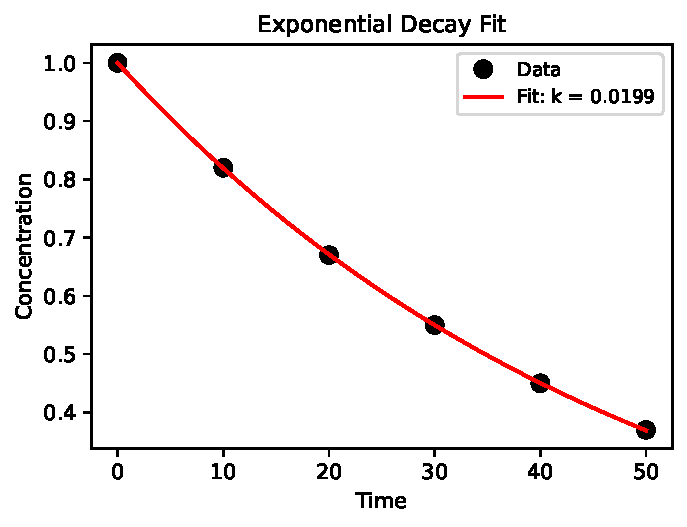
\includegraphics[width=0.7\textwidth]{figures/chap11/curve_fit_decay.pdf}
\end{center}

\begin{labexample}
Fitting a Gaussian peak to spectroscopy data:

\begin{lstlisting}
from scipy.optimize import curve_fit

def gaussian(x, amplitude, center, width, baseline):
    return amplitude * np.exp(-(x - center)**2 / (2 * width**2)) + baseline

# Simulated spectrum data
wavelengths = np.linspace(400, 600, 100)
true_peak = gaussian(wavelengths, 0.8, 500, 20, 0.1)
noise = np.random.randn(100) * 0.02
spectrum = true_peak + noise

# Fit
p0 = [0.7, 495, 25, 0.1]  # initial guesses
popt, pcov = curve_fit(gaussian, wavelengths, spectrum, p0=p0)

print(f"Peak center: {popt[1]:.1f} nm")
print(f"Peak width (sigma): {popt[2]:.1f} nm")
print(f"Peak amplitude: {popt[0]:.3f}")
\end{lstlisting}

\begin{center}
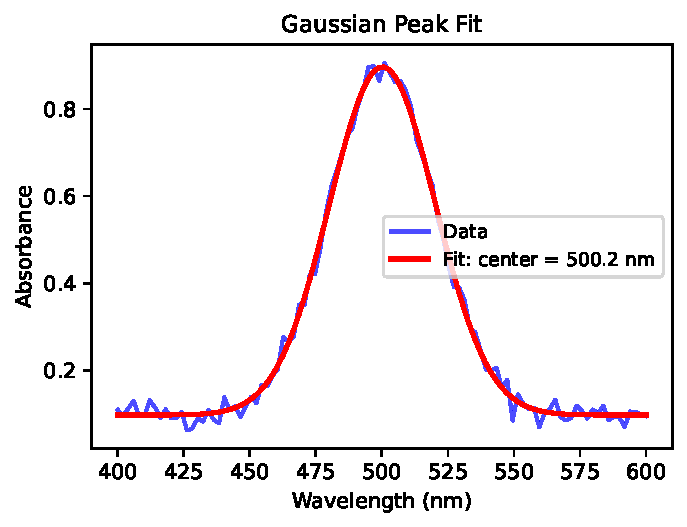
\includegraphics[width=0.7\textwidth]{figures/chap11/curve_fit_gaussian.pdf}
\end{center}
\end{labexample}

% ----------------------------------------------------------------------------
\section{Optimization}
\label{sec:optimization}

\subsection{Minimization}

\begin{lstlisting}
from scipy.optimize import minimize

# Function to minimize
def rosenbrock(x):
    return (1 - x[0])**2 + 100 * (x[1] - x[0]**2)**2

# Starting point
x0 = [0, 0]

# Minimize
result = minimize(rosenbrock, x0, method="Nelder-Mead")
print(f"Minimum at: {result.x}")
print(f"Minimum value: {result.fun}")
\end{lstlisting}

\subsection{Root Finding}

\begin{lstlisting}
from scipy.optimize import root_scalar, fsolve

# Find where f(x) = 0
def f(x):
    return x**3 - 2*x - 5

# Scalar root finding
result = root_scalar(f, bracket=[2, 3])
print(f"Root: {result.root:.6f}")

# Multiple equations
def equations(vars):
    x, y = vars
    return [x + y - 4, x * y - 3]

solution = fsolve(equations, [1, 1])
print(f"Solution: x={solution[0]:.4f}, y={solution[1]:.4f}")
\end{lstlisting}

% ----------------------------------------------------------------------------
\section{Integration}
\label{sec:integration}

\subsection{Definite Integrals}

\begin{lstlisting}
from scipy.integrate import quad

# Integrate sin(x) from 0 to pi
def f(x):
    return np.sin(x)

result, error = quad(f, 0, np.pi)
print(f"Integral: {result:.6f}")  # Should be 2.0

# With lambda
result, error = quad(lambda x: x**2, 0, 1)  # integral of x^2
\end{lstlisting}

\subsection{Differential Equations}

\begin{lstlisting}
from scipy.integrate import odeint

# First-order ODE: dy/dt = -k*y
def decay(y, t, k):
    return -k * y

k = 0.1
y0 = 1.0
t = np.linspace(0, 50, 100)

solution = odeint(decay, y0, t, args=(k,))

import matplotlib.pyplot as plt
plt.plot(t, solution)
plt.xlabel("Time")
plt.ylabel("Concentration")
\end{lstlisting}

\begin{center}
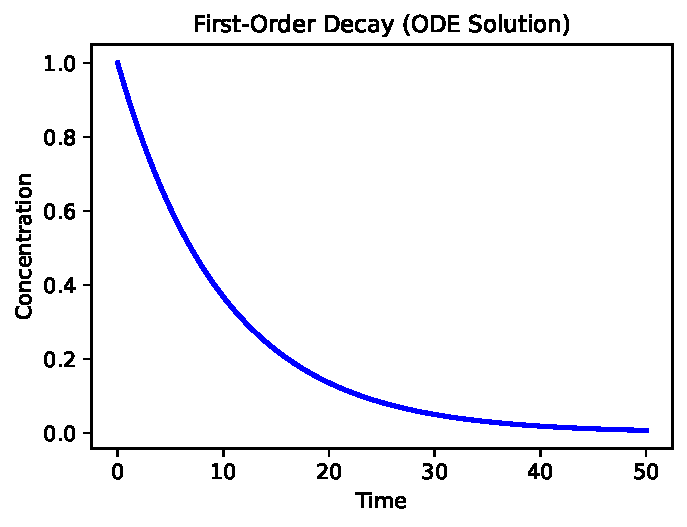
\includegraphics[width=0.7\textwidth]{figures/chap11/ode_decay.pdf}
\end{center}

\begin{labexample}
Solving coupled ODEs for a reaction A -> B -> C:

\begin{lstlisting}
from scipy.integrate import odeint

def reaction_system(y, t, k1, k2):
    A, B, C = y
    dAdt = -k1 * A
    dBdt = k1 * A - k2 * B
    dCdt = k2 * B
    return [dAdt, dBdt, dCdt]

# Parameters
k1, k2 = 0.1, 0.05
y0 = [1.0, 0.0, 0.0]  # initial: all A
t = np.linspace(0, 100, 200)

# Solve
solution = odeint(reaction_system, y0, t, args=(k1, k2))
A, B, C = solution.T

# Plot
plt.plot(t, A, label="A")
plt.plot(t, B, label="B")
plt.plot(t, C, label="C")
plt.xlabel("Time")
plt.ylabel("Concentration")
plt.legend()
\end{lstlisting}

\begin{center}
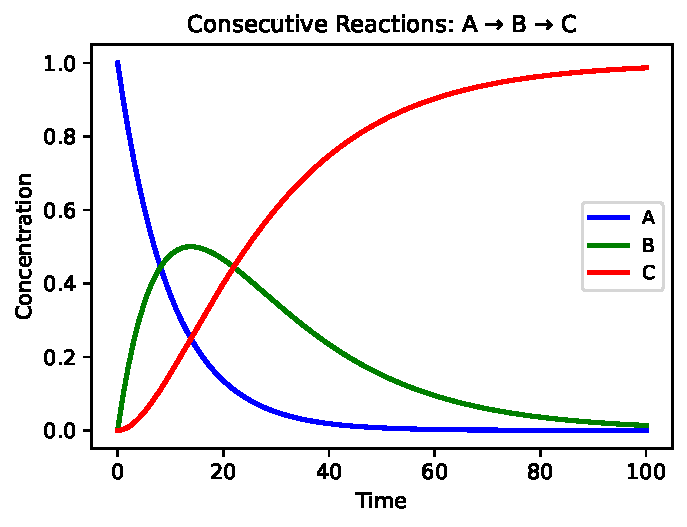
\includegraphics[width=0.7\textwidth]{figures/chap11/ode_reaction.pdf}
\end{center}
\end{labexample}

% ----------------------------------------------------------------------------
\section{Interpolation}
\label{sec:interpolation}

\begin{lstlisting}
from scipy.interpolate import interp1d

# Sparse data
x_data = np.array([0, 1, 2, 3, 4, 5])
y_data = np.array([0, 0.8, 0.9, 0.1, -0.8, -1.0])

# Create interpolation function
f_linear = interp1d(x_data, y_data, kind="linear")
f_cubic = interp1d(x_data, y_data, kind="cubic")

# Evaluate at new points
x_new = np.linspace(0, 5, 50)
y_linear = f_linear(x_new)
y_cubic = f_cubic(x_new)
\end{lstlisting}

\begin{center}
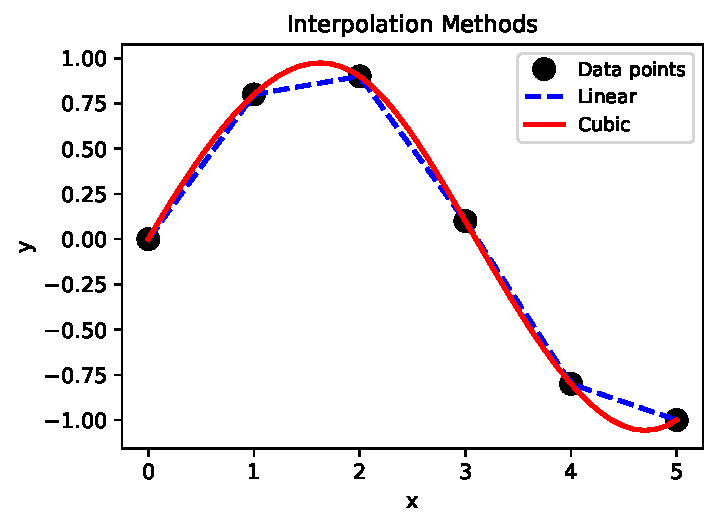
\includegraphics[width=0.7\textwidth]{figures/chap11/interpolation.pdf}
\end{center}

Interpolation types:
\begin{itemize}
    \item \py{"linear"}: straight lines between points
    \item \py{"cubic"}: smooth cubic spline
    \item \py{"nearest"}: step function
    \item \py{"quadratic"}: quadratic spline
\end{itemize}

% ----------------------------------------------------------------------------
\section{Signal Processing}
\label{sec:signal}

\subsection{Smoothing}

\begin{lstlisting}
from scipy.signal import savgol_filter
from scipy.ndimage import gaussian_filter1d

# Noisy data
x = np.linspace(0, 10, 100)
y_clean = np.sin(x)
y_noisy = y_clean + np.random.randn(100) * 0.2

# Savitzky-Golay filter
y_smooth = savgol_filter(y_noisy, window_length=11, polyorder=3)

# Gaussian smoothing
y_gauss = gaussian_filter1d(y_noisy, sigma=2)
\end{lstlisting}

\begin{center}
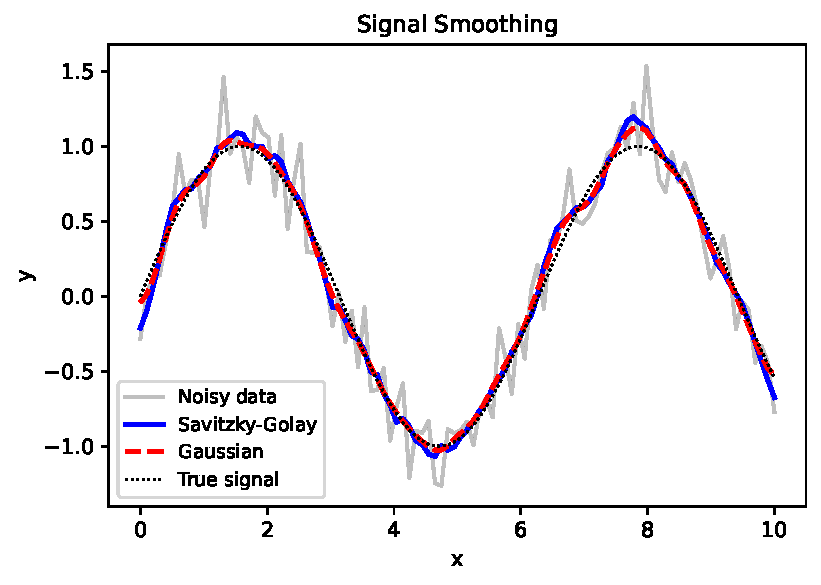
\includegraphics[width=0.7\textwidth]{figures/chap11/signal_smoothing.pdf}
\end{center}

\subsection{Peak Finding}

\begin{lstlisting}
from scipy.signal import find_peaks

# Find peaks
peaks, properties = find_peaks(y_data, height=0.5, distance=10)
print(f"Peak indices: {peaks}")
print(f"Peak heights: {properties['peak_heights']}")
\end{lstlisting}

\subsection{Fourier Transform}

\begin{lstlisting}
from scipy.fft import fft, fftfreq

# Time domain signal
dt = 0.01
t = np.arange(0, 1, dt)
signal = np.sin(2*np.pi*5*t) + 0.5*np.sin(2*np.pi*10*t)

# FFT
spectrum = fft(signal)
freqs = fftfreq(len(t), dt)

# Plot power spectrum
plt.plot(freqs[:len(freqs)//2], np.abs(spectrum[:len(spectrum)//2]))
plt.xlabel("Frequency (Hz)")
plt.ylabel("Amplitude")
\end{lstlisting}

\begin{center}
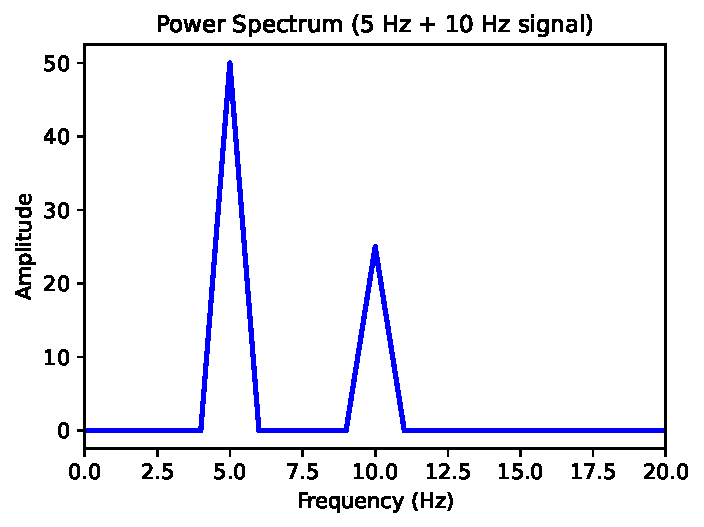
\includegraphics[width=0.7\textwidth]{figures/chap11/fft_spectrum.pdf}
\end{center}

% ----------------------------------------------------------------------------
\section{Special Functions}
\label{sec:special}

SciPy provides many mathematical special functions:

\begin{lstlisting}
from scipy import special

# Gamma function
special.gamma(5)       # 24.0 (= 4!)

# Error function
special.erf(1)         # 0.8427...

# Bessel functions
special.jv(0, 1)       # J_0(1) = 0.7652...

# Factorial
special.factorial(5)   # 120
\end{lstlisting}

% ----------------------------------------------------------------------------
\section{Physical Constants}
\label{sec:constants}

\begin{lstlisting}
from scipy import constants

constants.c           # speed of light (m/s)
constants.h           # Planck constant (J*s)
constants.k           # Boltzmann constant (J/K)
constants.R           # gas constant (J/(mol*K))
constants.N_A         # Avogadro number

# Convert units
constants.convert_temperature(100, "C", "K")  # 373.15
constants.calorie     # 1 calorie in Joules
\end{lstlisting}

% ----------------------------------------------------------------------------
\section{Chapter Summary}
\label{sec:scipy-summary}

SciPy extends NumPy with scientific algorithms:

\begin{itemize}
    \item \textbf{Statistics:} \py{stats.ttest\_ind()}, \py{stats.linregress()}, distributions
    \item \textbf{Curve fitting:} \py{optimize.curve\_fit()}
    \item \textbf{Optimization:} \py{optimize.minimize()}, \py{optimize.root\_scalar()}
    \item \textbf{Integration:} \py{integrate.quad()}, \py{integrate.odeint()}
    \item \textbf{Interpolation:} \py{interpolate.interp1d()}
    \item \textbf{Signal processing:} \py{signal.find\_peaks()}, \py{signal.savgol\_filter()}
    \item \textbf{Constants:} \py{constants.R}, \py{constants.N\_A}
\end{itemize}

\begin{ponder}
\begin{enumerate}
    \item When would you use \py{curve\_fit} vs. \py{linregress}?
    \item What's the difference between interpolation and curve fitting?
    \item How do you interpret a p-value from a t-test?
    \item Why might you need to provide initial guesses (\py{p0}) for curve fitting?
\end{enumerate}
\end{ponder}
